%==============================================================================
% sections/06_hidden_regular_variation.tex
%==============================================================================
\section{Hidden Regular Variation and Dependent Second-Order Terms}
\label{sec:hidden-rv}

\subsection{Why hidden cones matter}

Ordinary MRV may report asymptotic independence: the limiting spectral measure
is concentrated on coordinate axes. In that case the first-order tail constant
for \(S_N\) can look identical to the independent constant. This does not mean
that dependence is irrelevant at realistic thresholds. Joint-tail mass can live
on smaller cones at a slower scale. Hidden regular variation formalizes that
phenomenon and is especially relevant for financial data, where two factors may
rarely be extreme together but still co-crash often enough to affect 99.5\% or
99.9\% risk estimates.

\subsection{Cone decomposition and hidden regular variation}

For simplicity consider the positive loss cone. Let
\[
  \Eset_1=[0,\infty)^N\setminus\{0\}, \qquad
  \Eset_2=[0,\infty)^N\setminus\bigcup_{i=1}^N\{te_i:t>0\}.
\]
The first cone captures all extremes; the second removes the coordinate axes
and captures joint extremes.

\begin{definition}[Hidden regular variation]
\label{def:hrv}
Let $X$ be a non-negative random vector with $X\in\MRV(\alpha,\Gb,\nu_1,\Eset_1)$
and suppose $\nu_1$ is concentrated on the coordinate axes. We say that $X$
exhibits hidden regular variation on $\Eset_2$ with hidden tail scale $\Hb_2$
and hidden limit measure $\nu_2$, written $X\in\HRV(\alpha_2,\Hb_2,\nu_2,\Eset_2)$,
if $\Hb_2\in\RV_{-\alpha_2}$ with $\alpha_2\ge\alpha$ and
\[
  \frac{\Pb(X/x\in\cdot)}{\Hb_2(x)}\xrightarrow{v}\nu_2(\cdot)
  \quad\text{vaguely on }\Eset_2,
\]
with $\nu_2$ non-zero, homogeneous of order $-\alpha_2$, and supported on
$\Eset_2$. When $\alpha_2>\alpha$, $\Hb_2(x)=o(\Gb(x))$ but $\Hb_2$ may exceed
the marginal second-order scale $\Gb(x)|A(x)|$ or the mean-shift scale
$\Gb(x)/x$.
\end{definition}

Hidden regular variation in the sense of \cref{def:hrv} originates with
\citet{LedfordTawn1996}, \citet{Resnick2002}, and
\citet{MaulikResnick2005}; \citet{DasMitraResnick2013} emphasize the
empirical consequences for risk regions away from the axes. The combination
of an axis-supported first-order $\nu_1$ and a hidden $\nu_2$ on $\Eset_2$
formalizes the observation that two factors may rarely be jointly extreme but
co-crash often enough to affect 99.5\% and 99.9\% risk estimates.

\begin{assumption}[Ordered hidden-cone scale]
\label{ass:hidden-scale}
The first-order measure $\nu_1$ is axis-supported (i.e.\ assigns zero mass to
$\Eset_2$); $X$ exhibits hidden regular variation on $\Eset_2$ with scale
$\Hb_2$ and limit measure $\nu_2$ in the sense of \cref{def:hrv}; and the
risk-set boundaries for the sum functional are null under both $\nu_1$ and
$\nu_2$. Let
\[
  r(x)=\max\{\Hb_2(x),\Gb(x)|A(x)|,\Gb(x)/x\}.
\]
The remainder from triple and higher hidden cones not explicitly modeled is
$o(r(x))$, or those cones are absorbed into $\nu_2$ as block cones.
\end{assumption}

\begin{theorem}[Hidden-cone second-order expansion]
\label{thm:hidden-second-order}
Under \cref{ass:ind-sbj,ass:sote,ass:hidden-scale} with axis first-order
measure and hidden cone measure \(\nu_2\),
\[
  \Pb(S_N>x)
  = C_{\mathrm{axis}}\Gb(x)
    + D_{\mathrm{hid}}\Hb_2(x)
    + \Gb(x)A(x)D_{\mathrm{marg}}
    + \frac{\alpha\Gb(x)}{x}D_{\mathrm{mean}}
    + o(r(x)),
\]
where
\[
  D_{\mathrm{hid}}=\nu_2\{z:\sum_i z_i>1\},\quad
  D_{\mathrm{marg}}=\sum_{i\in\Aset}c_id_i,
  \quad
  D_{\mathrm{mean}}=\sum_{i\in\Aset}c_i\mu_{-i}.
\]
\end{theorem}

\begin{proof}[Proof sketch]
Split the risk set into an axis neighbourhood and the hidden-cone region
$\Eset_2$. The axis region contributes the marginal second-order and mean-shift
terms by the localization argument of \cref{thm:second-order}; the hidden
region contributes $\Hb_2(x)\nu_2(A_S\cap\Eset_2)$ by \cref{def:hrv}; the
overlap between the two regions is null by construction. The full argument is
in \cref{appx:second-hidden}.
\end{proof}

This theorem is a template result: the proof is rigorous once the cone scales
and boundary assumptions are verified for a concrete model. The planned
simulation designs include Gaussian copula asymptotic independence, selected
Archimedean copulas, and mixture models that create controllable hidden-cone
mass.

\subsection{Mixture estimator for axis and hidden cones}

A practical estimator should allocate effort to the axis event and to hidden
joint-tail events. Let \(Z_{\mathrm{axis}}(x)\) estimate the axis component and
\(Z_{\mathrm{hid}}(x)\) estimate the hidden-cone component. With mixture
probability \(\pi_x\), define
\[
  Z^{\mathrm{mix}}(x)
  =\frac{\1\{I=0\}}{\pi_x}Z_{\mathrm{axis}}(x)
   +\frac{\1\{I=1\}}{1-\pi_x}Z_{\mathrm{hid}}(x),
\]
where \(I\sim\mathrm{Bernoulli}(1-
\pi_x)\) is independent of the simulation draws. Choosing
\(\pi_x\) proportional to preliminary estimates of the axis and hidden
components gives a stratified estimator whose variance does not waste samples
on a cone that is negligible at the current threshold.

\begin{figure}[p]
\centering
\begin{figure}[t]
\centering
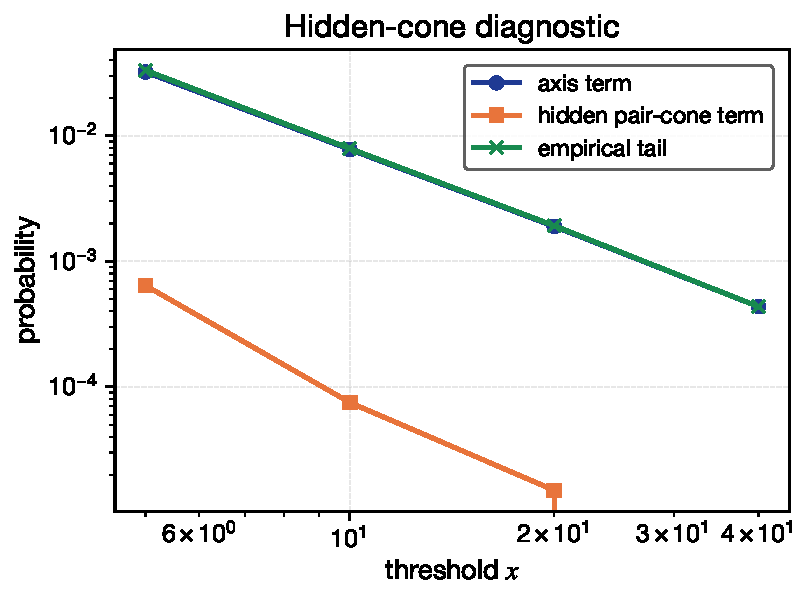
\includegraphics[width=0.85\linewidth]{figures/F13_hidden_cones_placeholder.pdf}
\caption[Hidden-cone diagnostic]{Axis exceedance term (blue), hidden pair-cone term (orange), and empirical sum-tail (green). The hidden-cone scale $\overline H_2(x) \propto x^{-\alpha_2}$ with $\alpha_2 = 3$ decays faster than the axis scale $\alpha = 2$, so the hidden term sits below the axis term at every threshold; the gap is the hidden-cone mass quantified by Theorem~\ref{thm:hidden-second-order}.}
\label{fig:hidden-cones-placeholder}
\end{figure}

\caption[Hidden-cone diagnostic]{Hidden-cone
diagnostic. The final figure will compare axis exceedances, pair-cone
exceedances, and block-cone exceedances across thresholds. It will report
whether the hidden scale is larger than the marginal second-order and
mean-shift scales over the empirical range. Source schema:
\texttt{results/F13\_hidden\_cones.csv}.}
\label{fig:hidden-cones-placeholder}
\end{figure}

\subsection{Empirical diagnostics for hidden variation}

The real-data analysis reports three hidden-cone diagnostics. First, for each
pair \((i,j)\), it estimates the Ledford--Tawn residual tail-dependence slope
from
\[
  \Pb(U_i>1-s,U_j>1-s)\approx L(s)s^{1/\eta_{ij}},
\]
where \(U_i\) are marginal ranks. Second, it estimates pair-cone exceedance
rates conditional on \(\|X\|>u\). Third, it compares pair-cone risk
contributions with the independent second-order correction at the VaR/ES
thresholds. The results populate \cref{tab:tail-dep-placeholder} and
\cref{fig:tail-dep-heatmap-placeholder}.
